\paragraph{Four-room development pilot.}
A new $16\times12$ m constructed four-room layout contains 16 objects and 121.48 m$^2$ of start-reachable free space. The frozen joint-exploration implementation starts from one rendered RGB-D/scan packet, with no movement prefix and 8.53\% initial coverage. The original 96-action budget and return contract are retained. Inputs include exact simulated odometry and ideal visible semantic labels; an explicit class-2/class-3 dictionary adapter reconciles the older scene generator with the v10 scorer. Hidden geometry is reserved for simulation and evaluation.

Both G and S execute 96 actions, travel 17.2 m, make ten turns, avoid simulated collisions and return to the start. Their coverage curves coincide and reach 39.84\%; neither reaches 90\% coverage. Actions first diverge at step 79, so equal coverage does not imply identical trajectories. This is one development layout with two paired runs, not a completed full-coverage benchmark or an observed semantic efficiency gain. The mapper's surface-patch counts do not measure reconstruction accuracy; the following extension evaluates TSDF quality against a separate exterior reference.

\begin{figure}[!htbp]
\centering
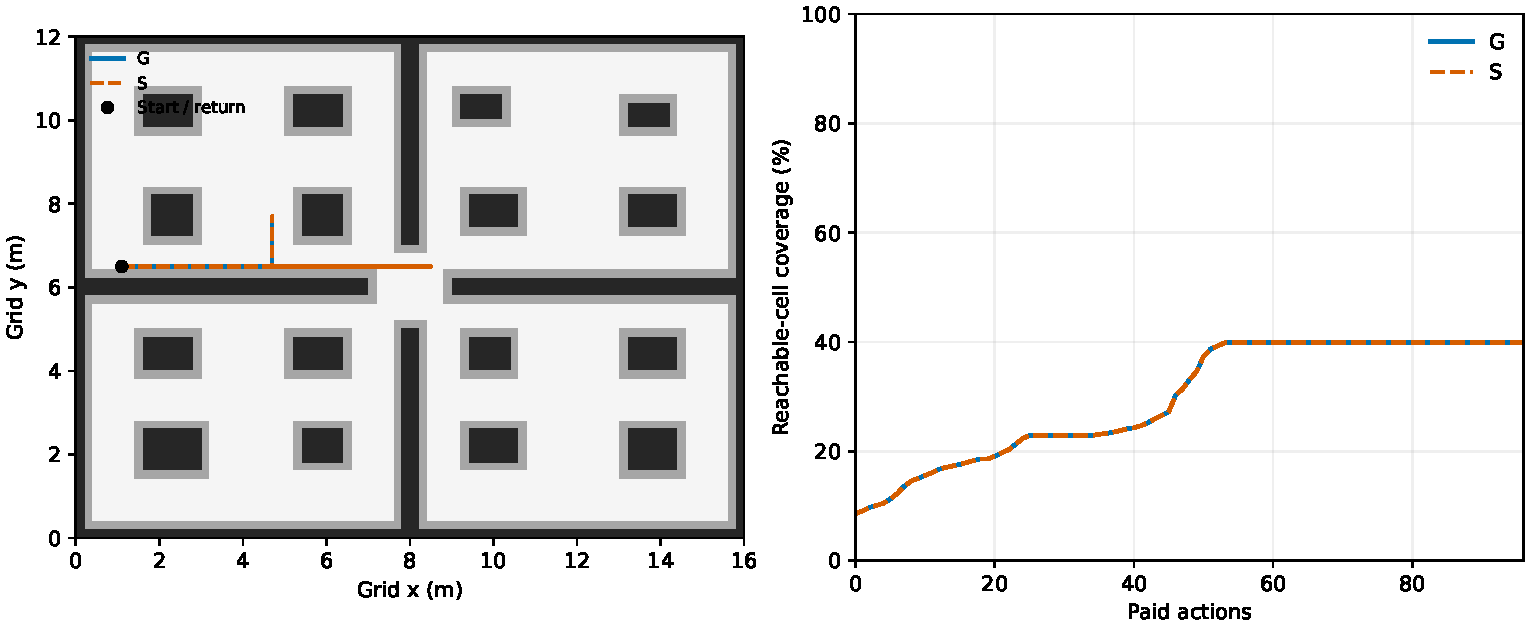
\includegraphics[width=\linewidth]{Unknown_rooms_20261119.pdf}
\caption{Four-room development pilot. Left: evaluator-only occupancy geometry and actual G/S trajectories; the full geometry is not supplied to the planner. Right: coverage measured on the same start-reachable free-cell reference after each paid action. The curves overlap from 8.53\% to 39.84\%, despite a late action difference. Both routes exhaust the 96-action budget and return.}\label{fig:nov19-unknown}
\end{figure}
